\documentclass[tikz]{standalone}
\usepackage{amsmath}
\usepackage{pgfplots}
\usetikzlibrary{arrows,intersections,math}

\begin{document}
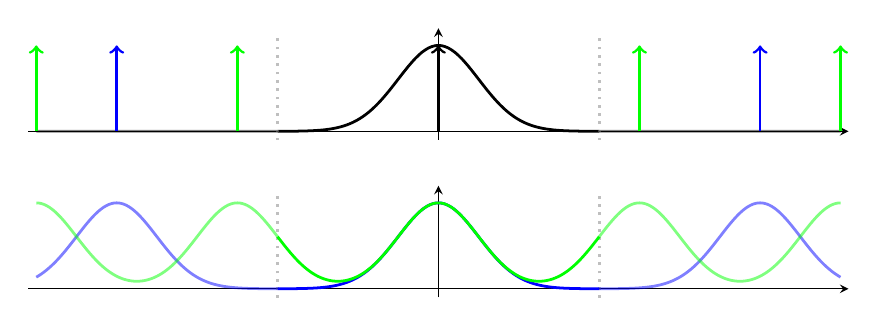
\begin{tikzpicture}
	\begin{scope}
	\begin{axis}[axis lines=middle, width=12cm, height=3cm,
		y label style={at={(axis cs:0.2, 1)},anchor=west},
		xmin=-10.2, xmax=10.2, ymin=-0.1, ymax=1.2, ytick={-2}, xtick={-20}]
		\addplot[domain=-10:-4, samples=50, smooth, line width=1pt, opacity=0.5] {exp(-(\x^2)/2)};
		\addplot[domain= -4:4,  samples=50, smooth, line width=1pt]              {exp(-(\x^2)/2)};
		\addplot[domain=  4:10, samples=50, smooth, line width=1pt, opacity=0.5] {exp(-(\x^2)/2)};
		
		\draw[line width=1pt, dotted, gray, opacity=0.5] (axis cs:-4,-0.4) -- (axis cs:-4,1.1);
		\draw[line width=1pt, dotted, gray, opacity=0.5] (axis cs: 4,-0.4) -- (axis cs: 4,1.1);
		
		\draw[line width=1pt, ->]       (axis cs:  0,0) -- (axis cs:  0,1);
		
		\draw[line width=1pt, ->, blue] (axis cs: -8,0) -- (axis cs: -8,1);
		\draw[line width=1pt, ->, blue] (axis cs:  8,0) -- (axis cs:  8,1);

		\draw[line width=1pt, ->,green] (axis cs:-10,0) -- (axis cs:-10,1);
		\draw[line width=1pt, ->,green] (axis cs: -5,0) -- (axis cs: -5,1);
		%\draw[line width=1pt, ->,green] (axis cs:  0,0) -- (axis cs:  0,1);
		\draw[line width=1pt, ->,green] (axis cs:  5,0) -- (axis cs:  5,1);
		\draw[line width=1pt, ->,green] (axis cs: 10,0) -- (axis cs: 10,1);
		
	\end{axis}
	\end{scope}
	\begin{scope}[yshift=-2 cm]
	\begin{axis}[axis lines=middle, width=12cm, height=3cm,
		xmin=-10.2, xmax=10.2, ymin=-0.1, ymax=1.2, ytick={-2}, xtick={-20}]
		
		\draw[line width=1pt, dotted, gray, opacity=0.5] (axis cs:-4,-0.4) -- (axis cs:-4,1.1);
		\draw[line width=1pt, dotted, gray, opacity=0.5] (axis cs: 4,-0.4) -- (axis cs: 4,1.1);

		\addplot[domain=-10:-4,samples=200, smooth, color=blue,line width=1pt, opacity=0.5] 
		{exp(-(\x^2)/2) + exp(-((\x+8)^2)/2) + exp(-((\x-8)^2)/2)};
		\addplot[domain=-4:4,samples=200, smooth, color=blue,line width=1pt] 
		{exp(-(\x^2)/2) + exp(-((\x+8)^2)/2) + exp(-((\x-8)^2)/2)};
		\addplot[domain=4:10,samples=200, smooth, color=blue,line width=1pt, opacity=0.5] 
		{exp(-(\x^2)/2) + exp(-((\x+8)^2)/2) + exp(-((\x-8)^2)/2)};
		
		\addplot[domain=-10:-4,samples=200, smooth, color=green,line width=1pt, opacity=0.5]
		{exp(-(\x^2)/2) + exp(-((\x+10)^2)/2) + exp(-((\x+5)^2)/2) + exp(-((\x-5)^2)/2) + exp(-((\x-10)^2)/2)};
		\addplot[domain=-4:4,samples=200, smooth, color=green,line width=1pt]
		{exp(-(\x^2)/2) + exp(-((\x+10)^2)/2) + exp(-((\x+5)^2)/2) + exp(-((\x-5)^2)/2) + exp(-((\x-10)^2)/2)};
		\addplot[domain=4:10,samples=200, smooth, color=green,line width=1pt, opacity=0.5]
		{exp(-(\x^2)/2) + exp(-((\x+10)^2)/2) + exp(-((\x+5)^2)/2) + exp(-((\x-5)^2)/2) + exp(-((\x-10)^2)/2)};
	\end{axis}
	\end{scope}
\end{tikzpicture}
\end{document}
